\section{Schrittweite}
Im folgenden Abschnitt wird die Schrittweite s konstant gew"ahlt, nur
der Gradient bestimmt die L"angen"anderung der gesamten Schrittweite.


\begin{figure}[h]
\centering
\begin{subfigure}[b]{0.49\textwidth}
\centering
%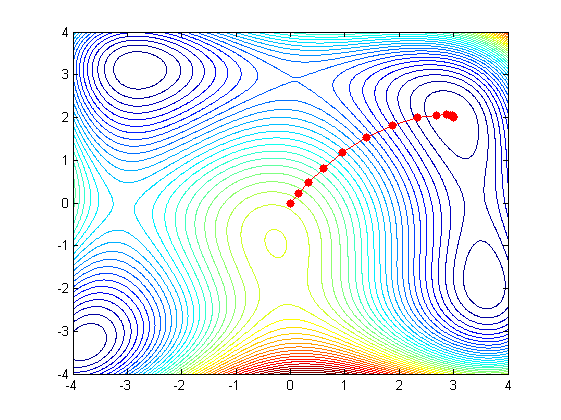
\includegraphics[width=\textwidth]{../bilder/himmelblau/HB_1.png}
\caption{s=0.01; n= 48}\label{schrittweite_a}
\end{subfigure} \begin{subfigure}[b]{0.49\textwidth}
\centering
%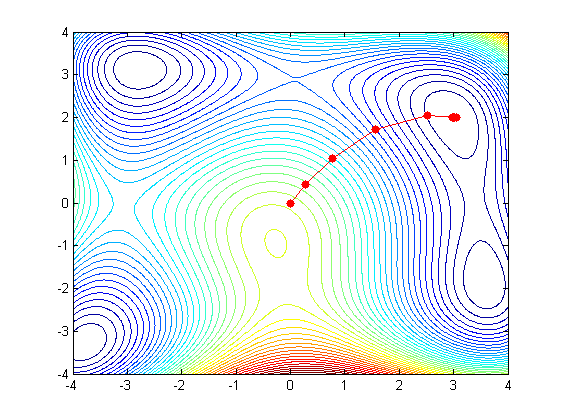
\includegraphics[width=\textwidth]{../bilder/himmelblau/HB_2.png}
\caption{s=0.02; n = 20}\label{schrittweite_b}
\end{subfigure}

\begin{subfigure}[b]{0.49\textwidth}
\centering
%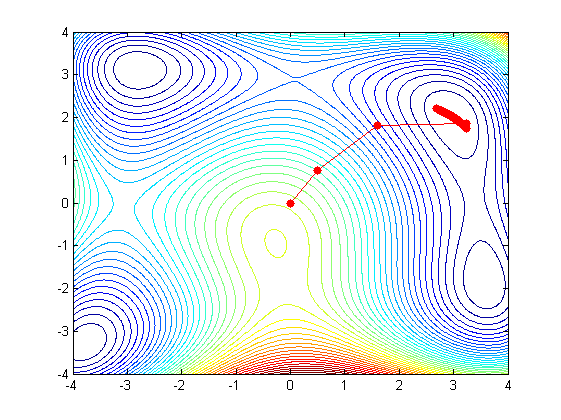
\includegraphics[width=\textwidth]{../bilder/himmelblau/HB_3.png}
\caption{s=0.035; n = 811}
\end{subfigure} \begin{subfigure}[b]{0.49\textwidth}
\centering
%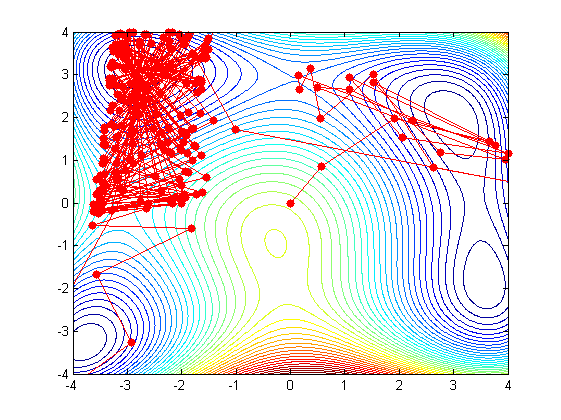
\includegraphics[width=\textwidth]{../bilder/himmelblau/HB_4.png}
\caption{s=0.0402; $n > 1000$}
\end{subfigure}
\caption{L"osungen mit verschiedene Schrittweiten}
\label{schrittweite}
\end{figure}

\figref{schrittweite_a} zeigt eine etwas langsame aber stetige Ann"aherung
an das lokale Minimum. Durch eine leichte Erh"ohung des $s$ wird die
Schrittweite und damit die Ann"aherungsgeschwindigkeit erh"oht (siehe
\figref{schrittweite_b} ).
In Abbildung c und d sind die Schrittweiten zu gross gew"ahlt und das Ziel
wird erst nach sehr vielen Iterationsschritten oder gar nicht erreicht.

Eine etwas anschaulichere Darstellung des Problems zeigt die nachfolgende
\figref{step}.
Die Abbildung zeigt klar, dass das $s$ weder zu klein noch zu gross gew"ahlt
werden darf. Das genaue Optimum zu finden ist jedoch sehr aufw"andig.

\begin{figure}
\centering
%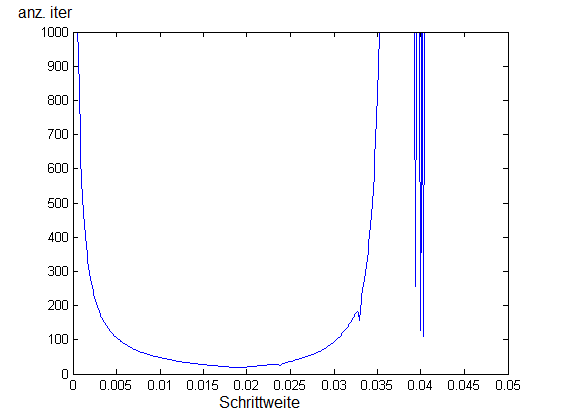
\includegraphics[height=0.6\textwidth]{../bilder/himmelblau/step.png}
\caption{Schrittweite zu Iterationsschritten}
\label{step}
\end{figure}
